% -- --------------------------------------------------------------------------------------------------- -- %
% -- Proyecto:                                                                                           -- %
% -- Archivo: reporte.rnw                                                                                -- %
% -- Repositorio: https://github.com/IFFranciscoME/A1_Temporal_Patterns                                  -- %
% -- Autor: Francisco ME                                                                                 -- %
% -- --------------------------------------------------------------------------------------------------- -- %

\documentclass{iteraposter}\usepackage[]{graphicx}\usepackage[]{color}
% maxwidth is the original width if it is less than linewidth
% otherwise use linewidth (to make sure the graphics do not exceed the margin)
\makeatletter
\def\maxwidth{ %
  \ifdim\Gin@nat@width>\linewidth
    \linewidth
  \else
    \Gin@nat@width
  \fi
}
\makeatother

\definecolor{fgcolor}{rgb}{0.345, 0.345, 0.345}
\newcommand{\hlnum}[1]{\textcolor[rgb]{0.686,0.059,0.569}{#1}}%
\newcommand{\hlstr}[1]{\textcolor[rgb]{0.192,0.494,0.8}{#1}}%
\newcommand{\hlcom}[1]{\textcolor[rgb]{0.678,0.584,0.686}{\textit{#1}}}%
\newcommand{\hlopt}[1]{\textcolor[rgb]{0,0,0}{#1}}%
\newcommand{\hlstd}[1]{\textcolor[rgb]{0.345,0.345,0.345}{#1}}%
\newcommand{\hlkwa}[1]{\textcolor[rgb]{0.161,0.373,0.58}{\textbf{#1}}}%
\newcommand{\hlkwb}[1]{\textcolor[rgb]{0.69,0.353,0.396}{#1}}%
\newcommand{\hlkwc}[1]{\textcolor[rgb]{0.333,0.667,0.333}{#1}}%
\newcommand{\hlkwd}[1]{\textcolor[rgb]{0.737,0.353,0.396}{\textbf{#1}}}%
\let\hlipl\hlkwb

\usepackage{framed}
\makeatletter
\newenvironment{kframe}{%
 \def\at@end@of@kframe{}%
 \ifinner\ifhmode%
  \def\at@end@of@kframe{\end{minipage}}%
  \begin{minipage}{\columnwidth}%
 \fi\fi%
 \def\FrameCommand##1{\hskip\@totalleftmargin \hskip-\fboxsep
 \colorbox{shadecolor}{##1}\hskip-\fboxsep
     % There is no \\@totalrightmargin, so:
     \hskip-\linewidth \hskip-\@totalleftmargin \hskip\columnwidth}%
 \MakeFramed {\advance\hsize-\width
   \@totalleftmargin\z@ \linewidth\hsize
   \@setminipage}}%
 {\par\unskip\endMakeFramed%
 \at@end@of@kframe}
\makeatother

\definecolor{shadecolor}{rgb}{.97, .97, .97}
\definecolor{messagecolor}{rgb}{0, 0, 0}
\definecolor{warningcolor}{rgb}{1, 0, 1}
\definecolor{errorcolor}{rgb}{1, 0, 0}
\newenvironment{knitrout}{}{} % an empty environment to be redefined in TeX

\usepackage{alltt}

\usepackage{lipsum}                                % Dummy text
\usepackage[absolute, overlay]{textpos}            % Figure placement
\setlength{\TPHorizModule}{\paperwidth}
\setlength{\TPVertModule}{\paperheight}


\title{
  Clustering subsecuencial de series de tiempo: Evidencia de patrones temporales en el
  tipo de cambio USD/MXN
  }

\vskip4cm

\author {
  Msc. Juan Francisco Mu\~noz Elguez\'abal \inst{1}
  \and
  Dr. Riemann Ru\'iz Cruz \inst{2}
  }

\institute {
  \inst{1} Msc. Ciencia de Datos - ITESO
  \and
  \inst{2} Departamento de Matem\'aticas y F\'isca - ITESO
  }

% -- --------------------------------------------------------------------------- Comienzo de codigo en R -- %










\IfFileExists{upquote.sty}{\usepackage{upquote}}{}
\begin{document}

\begin{frame}

\begin{columns}[onlytextwidth]

  \begin{column}{.7\textwidth - 0.01\textwidth}
    \begin{block}{Descripci\'on General}
      Metodolg\'ia \textit{BoxJenkins} para series de tiempo financieras. Modelo lineal 
      univariado que utiliza informaci\'on end\'ogena de la serie de tiempo para construir un modelo 
      matem\'atico con el cual realizar predicciones de valores futuros.
    \end{block}
    
    \begin{block}{Diagrama General}
      \begin{figure}[H]
        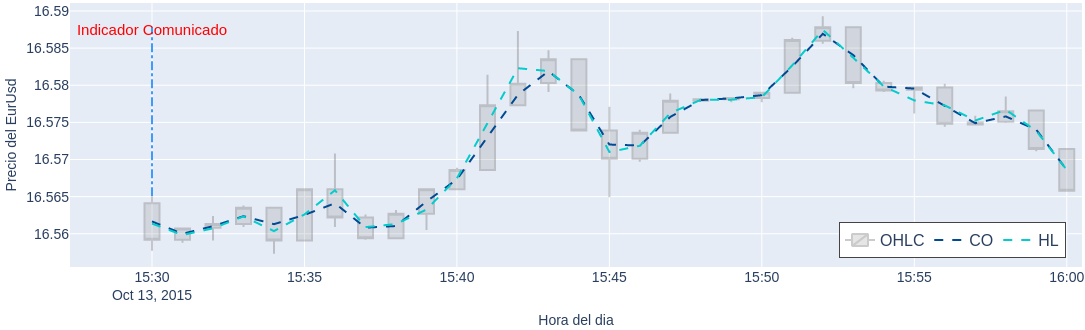
\includegraphics[scale=1]{imagenes/grafica_1.png}
      \end{figure}
    \end{block}
\end{column}

\begin{column}{.3 \textwidth - 0.01\textwidth}
  \begin{block}{Tabla General}
  \centering
     
\begin{tabular}{c|c|c|c}
\hline
categoria & usa & mex & total\\
\hline
actividad economica & 26 & 7 & 33\\
\hline
consumo & 29 & 5 & 34\\
\hline
energia & 4 & 0 & 4\\
\hline
flujos de capital & 5 & 0 & 5\\
\hline
inflacion & 0 & 4 & 4\\
\hline
mercado inmobiliario & 11 & 1 & 12\\
\hline
mercado laboral & 13 & 2 & 15\\
\hline
subasta de bonos & 5 & 0 & 5\\
\hline
tasas de interes & 1 & 1 & 2\\
\hline
total & 94 & 20 & 114\\
\hline
\end{tabular}


  \end{block}
\end{column}
  
\end{columns}


\end{frame}
\end{document}
